% SPDX-License-Identifier: AGPL-3.0-or-later
% Copyright (C) 2019-2025 Andrew Rechnitzer
% Copyright (C) 2022-2025 Colin B. Macdonald

\documentclass[12pt]{exam}

%%%%%%%%%%%%%%%%%%%%%%%%%%%%%%%%%%%%%%%%%%%%%%%%%%%%
%% This template uses latex exam class.
%%
%% This template is for letter-paper, not a4 paper.
%% The margins have been set so as to work nicely
%% with the QR-codes etc needed by Plom.
%%
%% It has also been designed to use the latex exam class
%% which auto-computes totals etc and also makes it easy
%% for the instructor to include solutions in their .tex
%% We recommend that you use this.

%%%%%%%%%%%%%%%%%%%%%%%%%%%%%%%
%% To print answers/soln and remove the extra spacing
%% just comment out the line below
%% vvvvvvv
%% vvvvv
%% vvv
%% v

\printanswers%

%% ^
%% ^^^
%% ^^^^^
%% ^^^^^^^
%% Try running this with and without the line above
%%%%%%%%%%%%%%%%%%%%%%%%%%%%%%%%%%%%%%%%%%%%%%%%%%%%
%% Add "draft" to show mock-up QR codes
%\usepackage{mockplom}
%\usepackage[draft]{mockplom}
%%%%%%%%%%%%%%%%%%%%%%%%%%%%%%%%%

\boxedpoints\addpoints\marksnotpoints%  % prefer 'marks' rather than 'points'
\extrawidth{-20mm}%

% Label questions as "Qn." rather than just "n."
\renewcommand{\questionlabel}{Q\thequestion.}

% A simple warning for your Do-Not-Mark pages
\newcommand{\dnm}{\noindent \emph{Please do not write on this page --- it will not be marked.}}

% Here are some handy commands for adding spacing / blank pages / answerboxes
% when printing with or without solns.

% Use this to put a vfill between things when printing
% without answers/solutions. No space when printing with answers/solns
\newcommand{\blank}{
  \ifprintanswers{}\else{\vfill}\fi
}

% Use this to put a blankpage when printing without answers/solutions.
% No page when printing with answers/solns
% This takes an optional argument of a question idx/number: \blankpage[X]
% and prints a message telling the student that this blank space is for
% question X. If no arg given then it prints the same message but for
% the current question.
\newcommand{\blankpage}[1][\thequestion]{
  \ifprintanswers{}\else{
  \par\vfill\newpage
  \noindent \emph{This blank page is for your solution to \textbf{Question~{#1}} if you need more space.}
  \par\vfill\newpage}\fi
}
% Thanks to PDL for improving the blankpage.

% Use this to make a nice answerbox which will display the correct answer
% when solutions are printed and is otherwise blank for the students
% to write their stuff.
\newcommand{\answerbox}[1]{
\begin{flushright}
\fbox{\parbox[l]{60mm}{Answer: \ifprintanswers{#1}\else{\vspace{10mm}}\fi}}
\end{flushright}
}
% A slightly larger answerbox
\newcommand{\Answerbox}[1]{
\begin{flushright}
  \fbox{\parbox[l]{80mm}{Answer: \ifprintanswers{#1}\else{\vspace{10mm}}\fi}}
\end{flushright}
}

%%%%%%%%%%%%%%%%%%%%%%%%%%%%%%%%%
%% Load packages and things here
\usepackage{amsmath,amsthm,amsfonts,amssymb}
\usepackage{enumerate}
\usepackage{graphicx}
\usepackage{tikz}

%%%%%%%%%%%%%%%%%%%%%%%%%%%%%%%%%
% Use tikz to put a big "Solutions" watermark on the first page
% if compiled with solutions
\newcommand{\watermarkPageIfSolutions}[1][\empty]{
\ifprintanswers%
\begin{tikzpicture}[remember picture, overlay]%
\node [text=red, rotate=55, scale=10, opacity=.25] at (current page.center){%
\ifx\empty{\textsf{SOLUTIONS}}\else{\begin{tabular}{c} \textsf{SOLUTIONS}\\ \textsf{VERSION~#1} \end{tabular}}\fi
};%
\end{tikzpicture}%
\fi%
}
% for demo purposes, we put a small watermark on each page using tikz
\AddToHook{shipout/background}[demoversion] {
\begin{tikzpicture}[remember picture, overlay]
  \node [below, text=teal, rotate=90, scale=3, opacity=.25] at (current page.west) {\textsf{demo version~2}};
\end{tikzpicture}
}


%%%%%%%%%%%%%%%%%%%%%%%%%%%%%%%%%
% Make the header blank, but put page info in the footer.
\chead{}
\cfoot{Page \thepage\ of \numpages}


%%%%%%%%%%%%%%%%%%%%%%%%%%%%%%%%%
%% Your macros should go here
%% for example
\newcommand{\dee}[1]{{\mathrm{d}#1}}
\newcommand{\diff}[2]{\dfrac{\dee{#1}}{\dee{#2}}}

%%%%%%%%%%%%%%%%%%%%%%%%%%%%%%%%%
%% Time to start the actual test

\begin{document}

\watermarkPageIfSolutions[2]%

\section*{Mathematics 418 --- Midterm --- 45 minutes}
\subsection*{3rd September 1752}
\begin{itemize}
	\item The test consists of \numpages\ pages and \numquestions\ questions worth a total of \numpoints\ marks.
	\item This is a closed-book examination. \textbf{None of the following are allowed}: documents, cheat sheets or electronic devices of any kind (including calculators, phones, smart watches, etc.)
	\item No work on this page will be marked.
	\item Fill in the information below before turning to the questions.
\end{itemize}
\bigskip
% be careful of changing position of ID box in this version.
% search for "y_offset" in launch_demo_bundle_creator.py
% and update accordingly.
\begin{center}
	\emph{This is the id page of ``version 2'' of the midterm; it is usually unused.}
\end{center}

\bigskip

\begin{center}
	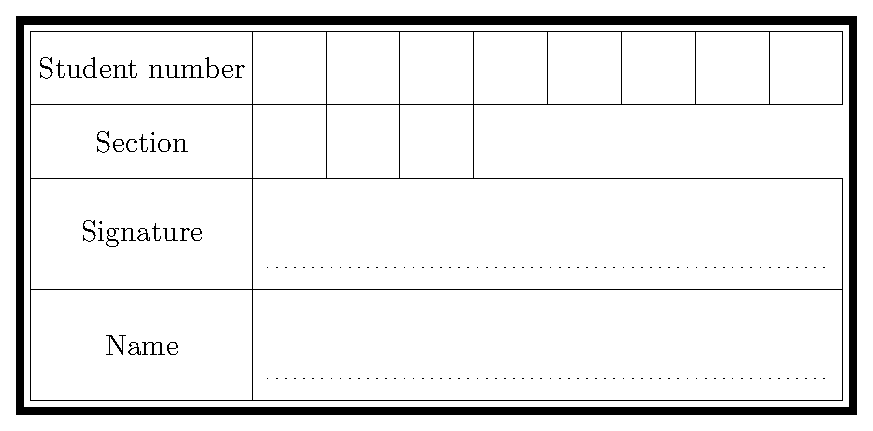
\includegraphics{idBox4}
\end{center}


\vfill
\newpage

\dnm%
\subsection*{Additional instructions}
\begin{itemize}
	\item Please use the spaces indicated.
	\item If you require extra paper then put up your hand and ask your instructor.
	      \begin{itemize}
		      \item You must put your name and student number on any extra pages.
		      \item You must indicate the test-number and question.
		      \item Please do this \textbf{on both sides} of any extra pages.
	      \end{itemize}
	\item Please do not dismember your test. You must submit all pages.
	\item Smoking is strictly prohibited during the test.
\end{itemize}

\vfill
\subsection*{Formula sheet}
You may find the following formulas useful in the questions that follow.
\begin{align*}
	a^2 + b^2           & = c^2                             \\
	e^{i\pi}+1          & = 0                               \\
	\sum_{i=1}^n i      & = \frac{n(n+1)}{2}                \\
	\diff{}{x}(f+g)     & = \diff{f}{x}+\diff{g}{x}         \\
	\int (f+g)\dee{x}   & = \int f \dee{x} + \int g \dee{x} \\
	\cos(a+b)           & = \cos a \cos b - \sin a \sin b   \\
	\sin(a+b)           & = \sin a \cos b + \cos a \sin b   \\
	A \cup (B \cap C)   & = (A\cup B) \cap (A \cup C)       \\
	A \cap (B \cup C)   & = (A\cap B) \cup (A \cap C)       \\
	\overline{A \cap B} & = \overline{A} \cup \overline{B}  \\
	\overline{A \cup B} & = \overline{A} \cap \overline{B}
\end{align*}
\vfill

\newpage


\begin{questions}
	\question[6]
	Compute the following limits.
	\begin{parts}
		\part\(\displaystyle \lim_{x \to 2} \dfrac{x^2-4}{x-2} \)
		\answerbox{4}
		\blank%
		\begin{solution}
			Notice that \( x^2-4 = (x-2)(x+2)\) and so
			\[
				\lim_{x \to 2} \dfrac{x^2-4}{x-2}
				= \lim_{x \to 2} \dfrac{(x-2)(x+2)}{x-2}
				= \lim_{x \to 2} (x+2)
				= 4
			\]
		\end{solution}
		\part\(\displaystyle \lim_{x \to +\infty} \dfrac{\sqrt{x^2+2x+3}}{2x-7} \)
		\answerbox{1/2}
		\blank%
		\begin{solution}
			First rewrite
			\[
				\dfrac{\sqrt{x^2+2x+3}}{2x-7}
				= \dfrac{|x|\sqrt{1 + 2/x +3/x^2}}{x(2-7/x)}
			\]
			Now since we take the limit to \(+\infty\) we can simplify this further
			\[
				\dfrac{\sqrt{x^2+2x+3}}{2x-7}
				= \dfrac{\sqrt{1 + 2/x +3/x^2}}{2-7/x}
			\]
			Hence
			\[
				\lim_{x \to +\infty} \dfrac{\sqrt{x^2+2x+3}}{2x-7}
				= \lim_{x \to +\infty} \dfrac{\sqrt{1+2/x+3/x^2}}{2-7/x}
				= 1/2
			\]
		\end{solution}
		\part\(\displaystyle \lim_{x \to 0^-} \dfrac{|x|}{x} \)
		\answerbox{-1}
		\blank%
		\begin{solution}
			Since we take the limit as \(x \to 0\) from below, we can simplify \(|x|=-x\), and hence
			\[
				\lim_{x \to 0^-} \dfrac{|x|}{x}
				= \lim_{x \to 0^-} \dfrac{-x}{x}
				= -1
			\]
		\end{solution}
	\end{parts}
	\newpage
	% for demo we label this question as Q(2)
	\renewcommand{\questionlabel}{Q(\thequestion)}
	\question[8] Compute the following derivatives:
	\begin{parts}
		\part\(\displaystyle \diff{}{x} \left(x^3 + 2x -\log(x) + 7 - \frac{1}{x} \right) \)
		\blank%
		\begin{solution}
			\begin{align*}
				\diff{}{x} \left(x^3 + 2x -\log(x) + 7 - \frac{1}{x}\right)
				 & = 3x^2 + 2 - \frac{1}{x} + 0 + \frac{1}{x^2}
			\end{align*}
		\end{solution}
		\part\(\displaystyle \diff{}{x} \left(x \sin(x)\right) \)
		\blank%
		\begin{solution}
			Using the product rule
			\begin{align*}
				\diff{}{x} x\sin(x) & = x \diff{}{x} \sin(x) + \sin(x) \diff{}{x}x \\
				                    & = x\cos(x) + \sin(x)
			\end{align*}
		\end{solution}
		\newpage
		\part\(\displaystyle \diff{}{x} e^{x^2} \)
		\blank%
		\begin{solution}
			Using the chain rule
			\begin{align*}
				\diff{}{x} e^{x^2} & = 2x e^{x^2}
			\end{align*}
		\end{solution}
		\part\(\displaystyle \diff{}{x} \left(\frac{x+2}{x-3}\right) \)
		\blank%
		\begin{solution}
			Using the quotient rule
			\begin{align*}
				\diff{}{x} \frac{x+2}{x-3} & = \frac{(x-3)\cdot \diff{}{x}(x+2) - (x+2)\diff{}{x}(x-3)}{(x-3)^2} \\
				                           & = \frac{x-3 - (x+2)}{(x-3)^2}                                       \\
				                           & = -\frac{5}{(x-3)^2}
			\end{align*}
		\end{solution}
	\end{parts}
	\newpage

	% for demo we label this question as Ex.3
	\renewcommand{\questionlabel}{Ex.\thequestion}
	\question[4]
	\begin{parts}
		\part\ Compute the cubic Taylor approximation of \(f(x)= \log(1+x) \) about \(x=0\).
		\blank\blank\blank%
		\begin{solution}
			We start by computing derivatives
			\begin{align*}
				f(x)    & = \log(1+x)          & f(0)    & = \log(1)= 0 \\
				f'(x)   & = \frac{1}{1+x}      & f'(0)   & = 1          \\
				f''(x)  & = -\frac{1}{(1+x)^2} & f''(0)  & = -1         \\
				f'''(x) & = \frac{2}{(1+x)^3}  & f'''(0) & = 2
			\end{align*}
			Then
			\[
				T_3(x) = 0 + x - \frac{x^2}{2} + \frac{x^3}{3}
			\]
		\end{solution}
		\part\ Hence estimate \( \log 2 \).
		\blank%
		\begin{solution}
			\begin{align*}
				\log 2 & \approx T_3(1) = 0 + 1 - \frac{1}{2} + \frac{1}{3} \\
				       & = \frac{6-3+2}{6} = \frac{5}{6}
			\end{align*}
		\end{solution}
	\end{parts}

	\newpage
	% for demo we label this question as LastQ
	\renewcommand{\questionlabel}{LastQ}
	\question[7] The mass of a sample of Polonium-210, initially 6 grams, decreases at a rate proportional to the mass. After one year, 1 gram remains.

	What is the half-life (the time it takes for the sample to decay to half its original mass)?
	\begin{solution}
		Let \(Q(t)\) denote the mass at time \(t\). We are told that $\diff{Q}{t}=-kQ$, where $k$ is a constant.

		We are told that
		\[
			Q(0)=6 \qquad Q(1)=1 \qquad \diff{Q}{t}=-kQ
		\]
		for some constant \(k>0\). Since this is a standard exponential growth/decay DE we know that
		\[
			Q(t) = C e^{-kt}
		\]
		Setting \(t=0\) gives us  \(Q(0)=C\) and then we also know that \(Q(1)=1\). Hence
		\begin{align*}
			1 & =Q(1)=6e^{-k(1)} & \text{ so} \\
			e^{-k}=1/6
		\end{align*}
		Putting everything together we get
		\[
			Q(t)=6(e^{-k})^t = 6^1 \cdot 6^{-t} = 6^{1-t}
		\]

		Now we need to find \(t\) so that \(Q(t)=Q(0)/2 = 3\)
		\begin{align*}
			3=Q(t) & =6^{1-t}                                                                             \\
			\log 3 & =(1-t)\log 6                                                                         \\
			1-t    & = \frac{\log 3}{\log 6}                                                              \\
			t      & = 1 - \frac{\log 3}{\log 6} = \frac{\log 6 - \log 3}{\log 6} = \frac{\log 2}{\log 6}
		\end{align*}
		The half-life of Polonium-210 is $\dfrac{\log 2}{\log 6}$ years.

	\end{solution}
	\blankpage%

\end{questions}
\end{document}
